In order to prove the correctness of the alloy model, some different real situation has been created by using the world predicates.
Here are the generated world replicas by predicates:
\begin{itemize}
    \item 
        \begin{figure}[H]
            \centering
            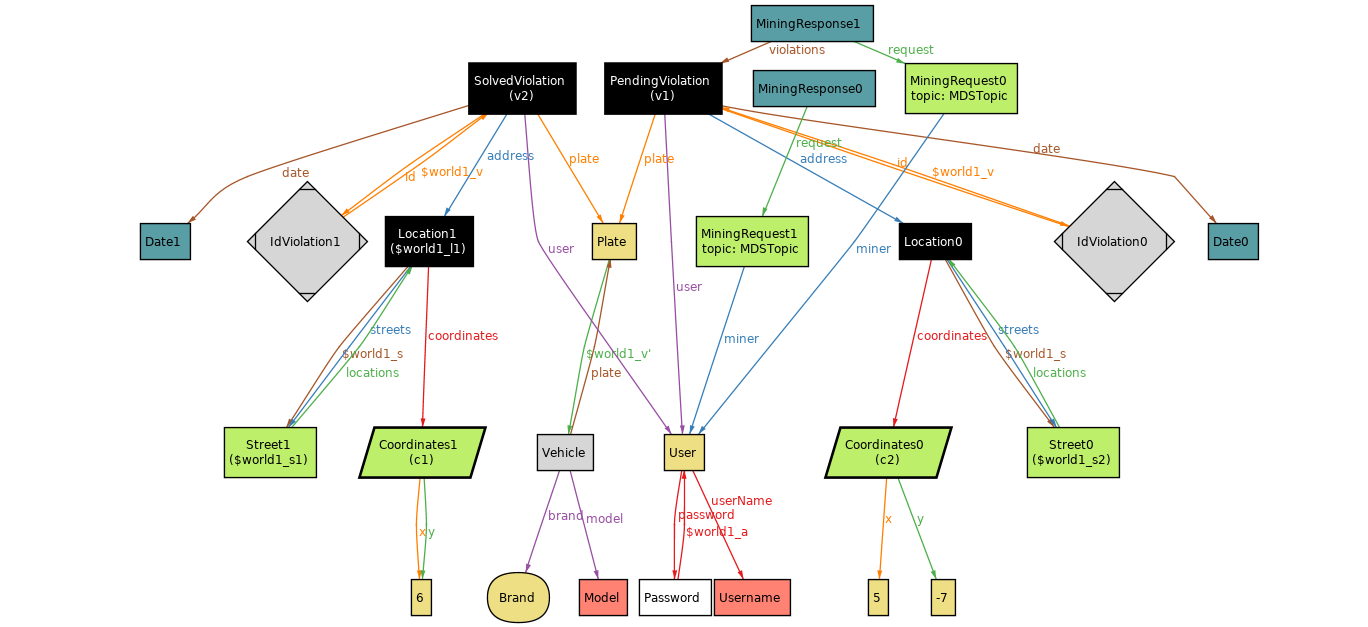
\includegraphics[width=1.0\textwidth]{alloy_world1}
            \caption{Alloy world 1}
            \label{fig:alloy_World1}
        \end{figure}
        \textit{World 1}: The first world pictures the situation in which a user publishes two different violation reports in different locations on different dates. Here is possible to underline the hierarchical relations between coordinates, locations and streets and the way reports are associated to users;
    \item 
        \begin{figure}[H]
            \centering
            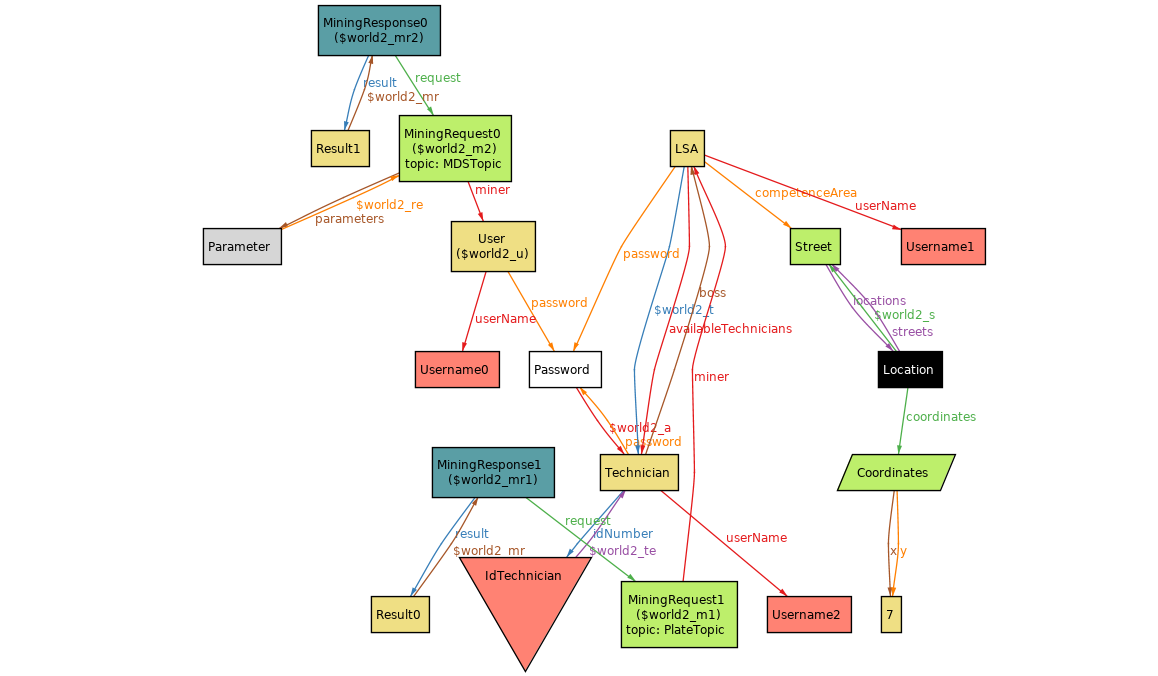
\includegraphics[width=1.0\textwidth]{alloy_world2}
            \caption{Alloy world 2}
            \label{fig:alloy_World2}
        \end{figure}
        \textit{World 2}: The second world pictures the situation in which different accounts have performed mining request on different topics. Here it is underlined that user can perform only MDS requests while technicians and LSAs can also be looking for Plate topics and deeper queries. Also, the number of parameters of each mining request have been limited to 3 for view purposes;
    \item 
        \begin{figure}[H]
            \centering
            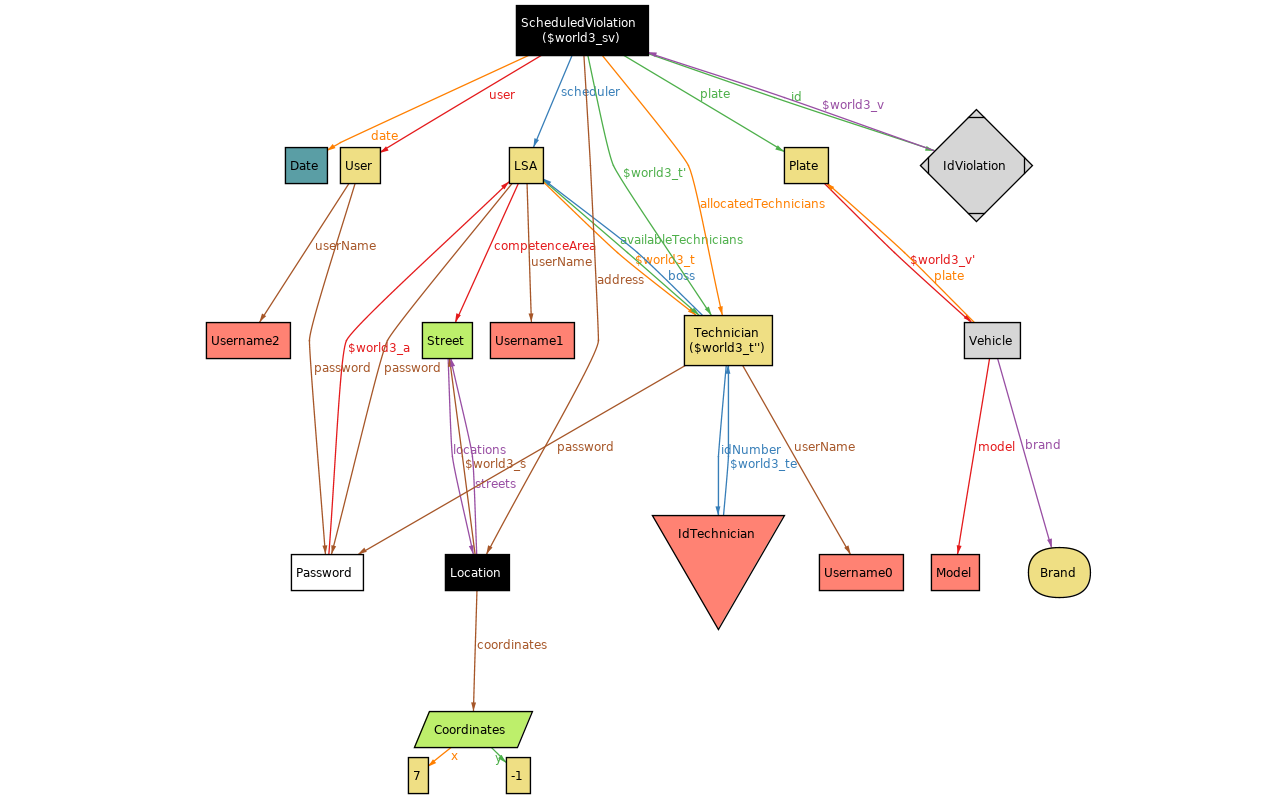
\includegraphics[width=1.0\textwidth]{alloy_world3}
            \caption{Alloy world 3}
            \label{fig:alloy_World3}
        \end{figure}
        \textit{World 3}: The third world pictures the situation in which a violation has been scheduled to a technician. Here the relations between technicians, scheduled violations and LSAs are underlined;
        \newpage
    \item 
        \begin{figure}[H]
            \centering
            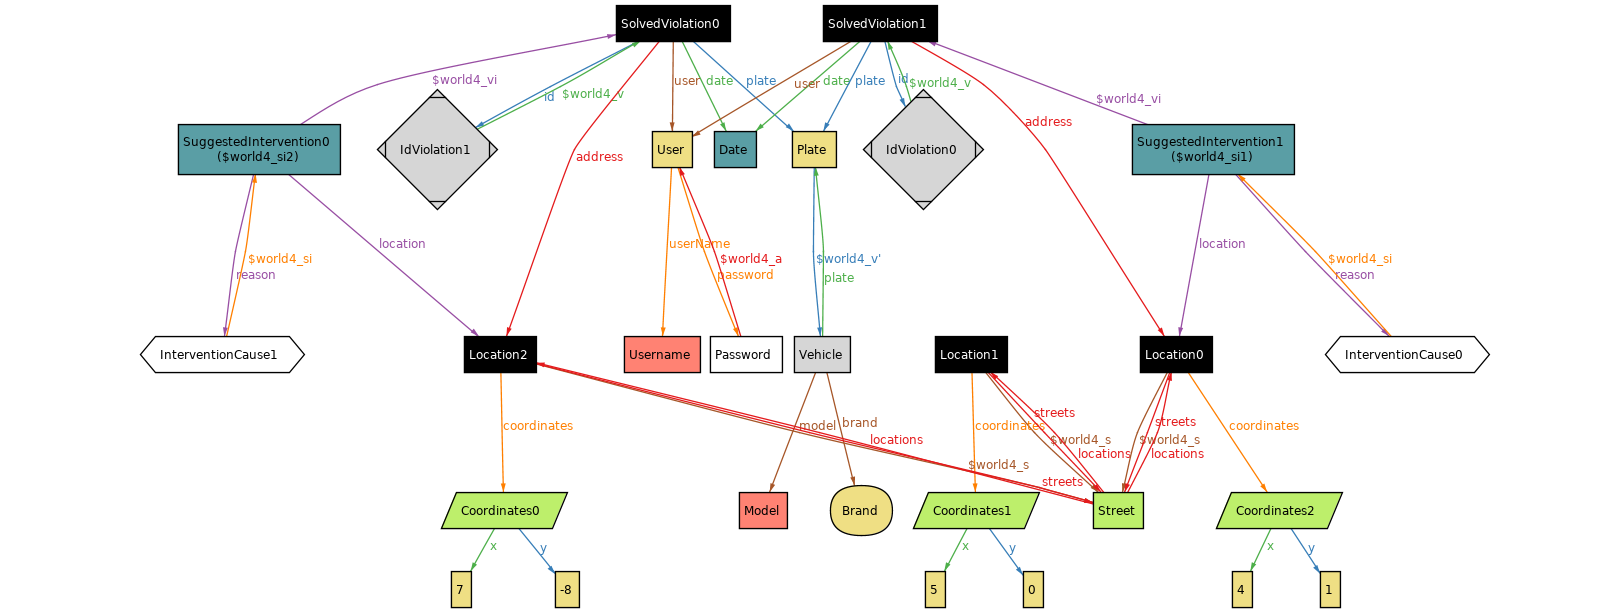
\includegraphics[width=1.0\textwidth]{alloy_world4}
            \caption{Alloy world 4}
            \label{fig:alloy_World4}
        \end{figure}
        \textit{World 4}: The fourth world pictures the situation in which a suggested intervention has been generated for a specific location. Here it is visible to have a look at the relations between suggested interventions, locations and violations. More specifically, it is possible to evince the fact that a suggested intervention can be performed on a certain location only if at least one violation occurred at the same spot.
\end{itemize}
